\documentclass[11pt,a4paper]{article}
\usepackage[utf8]{inputenc}
\usepackage{amsmath}
\usepackage{amsfonts}
\usepackage{amssymb}
\usepackage{enumitem}
\usepackage{listings}
\usepackage{xcolor}

\lstdefinelanguage{MySketch}%
{ mathescape,
  numbers=left,
  keywords={assume, assert, Array, Int, func, while,
  do, if, then, else, input, output, public, private, product, together, is,
  guard, instrument}
}

\definecolor{mGreen}{rgb}{0,0.6,0}
\definecolor{mGray}{rgb}{0.5,0.5,0.5}
\definecolor{mPurple}{rgb}{0.58,0,0.82}
\definecolor{backgroundColour}{rgb}{0.95,0.95,0.92}

\lstset{
    backgroundcolor=\color{backgroundColour},
    commentstyle=\color{mGreen},
    keywordstyle=\color{magenta},
    numberstyle=\tiny\color{mGray},
    stringstyle=\color{mPurple},
    basicstyle=\footnotesize,
    breakatwhitespace=false,
    breaklines=true,
    captionpos=b,
    keepspaces=true,
    numbers=left,
    numbersep=5pt,
    showspaces=false,
    showstringspaces=false,
    showtabs=false,
    tabsize=2,
    language=C
}

%%
%% Referencing in a space-saving manner
%%
\newcommand{\secref}[1]{\S\ref{sec:#1}}
\newcommand{\appref}[1]{Appendix~\ref{sec:#1}}
\newcommand{\subsecref}[1]{\S\ref{subsec:#1}}
\newcommand{\figref}[1]{Fig.~\ref{fig:#1}}
\newcommand{\algref}[1]{Alg.~\ref{alg:#1}}
\newcommand{\tabref}[1]{Table~\ref{tab:#1}}

\title{Review: Verifying Constant-Time Implementations}
%\subtitle{Formal Verification Background Paper Report}
\author{Mahyar Emami, Rishabh Iyer, Sahand Kashani \\ firstname.lastname@epfl.ch}

\begin{document}
\maketitle

\section{Introduction}
% Say a few general words about the general context of the paper you chose. Explain why the topic is of interest, or where it can be applied. If it is about a piece of software or artifact, give a description of it. State the main result of the paper and why it is new or how it improves on previous state of knowledge. You can cite references using, for example \cite{BibliographyManagementLaTeX} and make a succint presentation of the organisation of your report.

Timing attacks---attacks that extract secrets by measuring timing differences under adversary-controlled inputs---on cryptographic libraries~\cite{bernstein_cache_timing_attacks, dsa_exponentiations} pose a major challenge to information security today. 
Popular cryptographic libraries (e.g., OpenSSL~\cite{openssl}) run on millions of devices; hence a vulnerability in such a library has the potential to compromise all such devices simultaneously.

Constant-Time programming is the most effective software countermeasure against such attacks.
Constant-time programming involves rewriting a program such that (1)~its control flow does not depend on program secrets, (2)~it does not perform any secret-dependent memory accesses, and (3)~it does not use variable-latency instructions to operate on secrets.

However, it is challenging to write and/or reason about constant-time programs are hard since it typically involves the use of low-level programming languages and programming practices that deviate from software engineering principles.
For example, two constant-time violations\footnote{See pull requests \#147 and \#179 in ~\cite{s2n}} were found in Amazon's s2n library~\cite{s2n}soon after its release with the second exploiting a timing-related vulnerability introduced when fixing the first.

In this work, Almeida et. al~\cite{almeida} propose using formal methods to \emph{automatically} verify whether a program runs in constant time. 
To do so, they provide a precise framework to model constant-time properties(~\secref{prelimnaries}), a sound and complete reduction of constant-timeliness of input programs to assertion safety of a self-product(~\secref{body}) and design, evaluate an automated tool that verifies the constant-timeliness of cryptographic algorithms from widely used libraries within seconds(~\secref{eval}). 


\section{Preliminaries}

% State the technical details that are necessary to understand the paper. It is generally a collection of definitions, concepts and notations with potentially a few preliminary results. It can be, for example the mathematical framework in which the topic of your paper is expressed. In particular, fix the notation you will be using for your review.

\begin{itemize}
  \item Simple example that can easily be checked + example of benign branch that other tools cannot determine to be constant-time.
  \item Formalism used to model a program (while-language framework and what it supports).
  \item The paper proposes modeling contant-time verification of a program by encoding the input program as a safety condition and executing the program to check if it is safe.
  \item Define what leakage $L(c)$ is formally. A leakage model can either depend on
        \item \begin{enumerate}
          \item Path-based characterizaion of constant-time: leakage of branch conditions.
          \item Cache-based characterization of constant-time: leakage of memory access indices.
          \item Instruction-based characterization of constant-time: leakage of instruction operand sizes.
        \end{enumerate}
  \item Define what it means for a program to be safe (i.e., it does not violate an assertion inserted when the safety program).
\end{itemize}


\section{Redcuing security to safety}

% Explain the paper, in your own words. Don't go into as many details as the
% original text, but the person reading your review should have a general
% understanding of the paper's results and how those results can be obtained.
% The structure and content of this section of course heavily depends on the
% paper itself. Don't hesitate to split it in multiple sections or subsections,
% for example: \subsection{An algorithm for whatever problem we try to solve} If
% your paper contains theorems, sketch the proofs of important theorems.

% \subsection{Benchmarks} If it contains benchmarks, show the key scores or
% results.

% You can follow the structure of the paper you're reviewing, but write with
% your own words.

% \subsection{Reducing security to safety}

At the interface of any security-sensitive function call, there usually exists a
\emph{contract} that describes which inputs or outpus are deemed public (i.e.,
known to attackers) and which ones are private (i.e., to protect). A leak should
never reveal anyting about the private inputs and outputs (but publics ones 
can be leaked).
% If we denote a program as $p$ (with the usual definition of a prgram being a
% sequence of statements or programs) with a corresponding state $s$ (which
% is mapping from variables to values) then at each step of execution, from
% state $s$ executing program/statement $p$ we can define leakage $L(.)$ as follows:

% \begin{equation}
%     \begin{split}
%     L(\langle s, \text{\texttt{if}}~e~\text{\texttt{then}}~p_1~\text{\texttt{else}}~p_2 \rangle) = & s(e) \\
%     L(\langle s, \text{\texttt{while}}~e~\text{\texttt{do}}~p \rangle) = & s(e) \\
%     L(\langle s, x_0[e_0] = e \rangle) = & s(e_0)s(e_1)...s(e_n)
%     \end{split}
% \end{equation}

% The first two leakage sources correspond to leakage from control flow while the
% latter is leakage from memory access. Note that in the third leakage source,
% a memory leak $s(e_0)$ corresponds to leakage from the right-hand-side indexer
% expression and $s(e_1)$ to $s(e_n)$ possible indexer expression in expression
% $e$. We can also extend the leakage sources to comprise machine operations that
% have operand-dependent execution latency (i.e., division in x86).

Using the leakage rules in \secref{prelimnaries}, 
we can reduce constant-time security to execution safety (i.e., termination
without any failed assertions) by building a \emph{self-product} in which two
abstract execution take place back to back, only differing in the value of
private inputs and outputs. \figref{rules} shows how a program product can
be constructed where $\hat{p}$ is the program $p$ with all variables renamed
(i.e., an alternative execution).

\begin{figure}[h]
    \centering
    \subfigure[Program product construction rules]{
        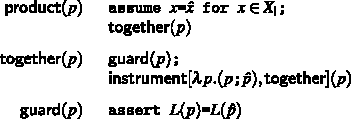
\includegraphics[width=0.45\textwidth]{./figs/fig_7.pdf}
    }\label{fig:fig_7}
    \subfigure[Instrumentation rules] {
        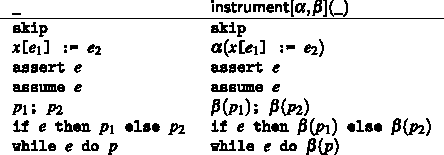
\includegraphics[width=0.45\textwidth]{./figs/fig_8.pdf}
    }\label{fig:fig_8}
    \caption{Program product}
    \label{fig:rules}
\end{figure}

\begin{figure}[t]
    \lstinputlisting[language=C]{example.c}
    \caption{Running example - sub-array copy}
    \label{fig:example}
  \end{figure}

The essence of the transformation is the instrumentation, which reduces 
constant-time security to assertion safety. \figref{example_prod} shows 
the product of the sub-array copy program in \figref{example}. Notice how
the program is instrumented with assertions to ensure leakage remains the same at
every step of execution. In this example, the private inputs \texttt{l\_idx} and
its renaming are not assumed to be equal, therefore the assetion on line 8 fails
and the program is proved to be unsafe and hence it follows that the program is
not constant-time secure.

\begin{figure}[h]
    \lstinputlisting[language=MySketch]{prod.my}
    \caption{example program product of the sub-array copy program.}
    \label{fig:example_prod}
\end{figure}



\section{Takeaways}

This work formalizes the previously imprecise notion of constant-time programming, in addition to providing a publicly available and fully automated tool can verify (in seconds) whether implementations of cryptographic algorithms from off-the-shelf libraries adhere to the notion of constant-time. 
This is, undoubtedly, an impressive result.

That said, the paper does have a few weaknesses: \\
\indent Firstly, \texttt{ct-verif} requires LLVM implementations which is problematic for two reasons.
Cryptographic code is often written directly in assembly due to the performance benefits. For instance, Vale~\cite{vale} demonstrates that OpenSSL assembly implementations outperform their C counterparts by up to 50\%.
Further, verifying that LLVM code runs in constant-time does not guarantee that the executable runs in constant time~\cite{KaufmannPVV16}. To the authors' credit, they do discuss such scenarios.

Secondly, the formalization of constant-time as presented by the papers is significantly weakened by the advent of micro-architectural attacks (~\cite{meltdown,spectre}). To be fair to the authors, such attacks became popular after their paper was published. Further, one could argue that such attacks are not a property of the implementation per-se, and are a menace that the underlying hardware/operating system must tackle.

Finally, the authors do not present a single example where their ``automated'' approach fails to verify constant-timedness in reasonable time. As such, the results look a little too good to be true. 

During the course of this project, we plan to investigate the first and third aspects of \texttt{ct-verif} more thoroughly. 
Specifically we aim to identify where the tool falls short and also patch it with LLVM-passes that can preserve constant-timedness. 

\bibliographystyle{plain}

\bibliography{biblio.bib}

\end{document}
